% REMEMBER: You must not plagiarise anything in your report. Be extremely careful.

\documentclass{l4proj}

    
%
% put any additional packages here
%

\begin{document}

%==============================================================================
%% METADATA
\title{Level 4 Project Report Template}
\author{John H. Williamson}
\date{September 14, 2018}

\maketitle

%==============================================================================
%% ABSTRACT
\begin{abstract}
    Every abstract follows a similar pattern. Motivate; set aims; describe work; explain results.
    \vskip 0.5em
    ``XYZ is bad. This project investigated ABC to determine if it was better. 
    ABC used XXX and YYY to implement ZZZ. This is particularly interesting as XXX and YYY have
    never been used together. It was found that  
    ABC was 20\% better than XYZ, though it caused rabies in half of subjects.''
\end{abstract}

%==============================================================================

% EDUCATION REUSE CONSENT FORM
% If you consent to your project being shown to future students for educational purposes
% then insert your name and the date below to  sign the education use form that appears in the front of the document. 
% You must explicitly give consent if you wish to do so.
% If you sign, your project may be included in the Hall of Fame if it scores particularly highly.
%
% Please note that you are under no obligation to sign 
% this declaration, but doing so would help future students.
%
%\def\consentname {My Name} % your full name
%\def\consentdate {20 March 2018} % the date you agree
%
\educationalconsent


%==============================================================================
\tableofcontents

%==============================================================================
%% Notes on formatting
%==============================================================================
% The first page, abstract and table of contents are numbered using Roman numerals and are not
% included in the page count. 
%
% From now on pages are numbered
% using Arabic numerals. Therefore, immediately after the first call to \chapter we need the call
% \pagenumbering{arabic} and this should be called once only in the document. 
%
% Do not alter the bibliography style.
%
% The first Chapter should then be on page 1. You are allowed 40 pages for a 40 credit project and 30 pages for a 
% 20 credit report. This includes everything numbered in Arabic numerals (excluding front matter) up
% to but excluding the appendices and bibliography.
%
% You must not alter text size (it is currently 10pt) or alter margins or spacing.
%
%
%==================================================================================================================================
%
% IMPORTANT
% The chapter headings here are **suggestions**. You don't have to follow this model if
% it doesn't fit your project. Every project should have an introduction and conclusion,
% however. 
%
%==================================================================================================================================
\chapter{Introduction}

% reset page numbering. Don't remove this!
\pagenumbering{arabic} 


\section{Concurrency and Distributed Systems}
Concurrency and distributed systems are becoming increasingly important in modern computational science, especially in the context of cloud computing and big data. \colorbox{yellow}{referenceHere[11]}Sutter and Larus (2005) emphasize that with the proliferation of multicore processors, the software industry needs to adopt new tools and ways of thinking in order to fully utilize the potential of multicore processors. Concurrency refers to the ability of a system to handle multiple tasks at the same time, which allows efficient use of computational resources. For example, by processing hundreds or even thousands of client requests in parallel, modern Web servers are able to dramatically improve response times and system throughput. This shift in demand requires mainstream software development to stop ignoring concurrency, a challenge that requires developers to master the design and implementation of concurrent programs (Sutter & Larus, 2005)\colorbox{yellow}{referenceHere[11]}.
    
The design of Multiplayer Online Role-Playing Game (MMORPG) servers, such as exemplified by the \colorbox{yellow}{referenceHere[7]}World of Warcraft (Figure \ref{fig:WoWlogo}) demonstrates the value of concurrent programming in real-world applications, where the use of a client-server model and event-driven architecture enables asynchronous processing of player requests. \colorbox{yellow}{referenceHere[9]}Kim and Kim's (2019) study, by utilizing Input/Output Completion Port (IOCP) and multithreading techniques, has demonstrated methods to effectively improve server performance, handle concurrent connections and employ fine-grained locking mechanisms for access control of shared resources to reduce the risk of deadlock and effectively improve system responsiveness and throughput.

\begin{figure}[h]
    \centering
    \begin{minipage}[t]{0.35\textwidth}
        \centering
        
\includegraphics[width=\linewidth,height=5cm,keepaspectratio]{images/WoWlogo.png}
        \caption{World of Warcraft}
        \label{fig:WoWlogo}
    \end{minipage}
    \quad
    \begin{minipage}[t]{0.30\textwidth}
        \centering
        \includegraphics[width=\linewidth,height=5cm,keepaspectratio]{images/PokemonGo.jpeg}
        \caption{Pokemon GO}
        \label{fig:PokemonGo}
    \end{minipage}
\end{figure}

On the other hand, Distributed systems achieve workload decentralization by assigning tasks across multiple compute nodes, which is especially critical for processing large-scale data sets. For example, \colorbox{yellow}{referenceHere[8][1]}Google's Bigtable and Apache Hadoop's Distributed File System (HDFS) are capable of handling petabytes of data and supporting complex data analysis tasks. In this context, the distributed architecture of \colorbox{yellow}{referenceHere[13]}Pokemon GO(Figure \ref{fig:PokemonGo}) demonstrates the efficient ability of distributed systems to manage and synchronize millions of players globally, through a network of servers deployed in multiple locations around the world, and the use of geo-distributed database technology to decentralize the storage of data based on the geographic location of players, showing the importance of this technology in dealing with large-scale, real-time interactive applications.
		
The combination of concurrency and distributed systems not only greatly improves the efficiency of task processing, but also enhances the reliability and scalability of the system. In the case of distributed databases, for example, data is replicated across multiple nodes, ensuring that the entire system can maintain normal operation even if some of the nodes fail. In addition, this technology supports the dynamic adjustment of computing resources according to actual demand, a feature that is widely used in cloud service platforms such as \colorbox{yellow}{referenceHere[2][10]}Amazon Web Services and Microsoft Azure. This exposition not only demonstrates the key role of concurrent programming in ensuring high availability and optimizing user experience, but also provides an important reference for designing efficient concurrent and distributed systems.

\section{Challenges}

While these systems are capable of handling unprecedented amounts of data and computational tasks, they also introduce a new set of challenges. 

\subsection{Thread Deadlock}

A commonly encountered problem in concurrent programming is thread deadlock, Holt (1972) \colorbox{yellow}{referenceHere} defines that when a process P in a system is blocked in state S and there does not exist any state T such that S can transition to T, then we say that process P is in a deadlocked state in state S. A process P is considered deadlocked if it is blocked in T for all possible states T . For example, a deadlock is caused when two threads have each locked some resources and are both waiting for the other to release their holdings. This situation is particularly common in database transaction processing and operating system resource allocation, and seriously affects program stability and efficiency.

\subsection{Communication Mismatch}

Communication mismatch is another critical issue in distributed systems. Nodes in a distributed environment need to exchange information frequently, and any inconsistency in communication protocols or data formats can lead to major failures. Taking microservice architecture as an example, if the communication interfaces between services are not clearly defined or fail to maintain compatibility during version updates, it may lead to the functional failure of the whole system. This is particularly noticeable in fast iterative and multi-team projects and requires special attention.

\section{Case Study: The Mailbox Mechanism}

In further exploring the application of the Pat language in the field of concurrent programming, this paper aims to show how mailbox types in the Pat language can effectively manage concurrent tasks by introducing a concrete code example. As we see in Listing \ref{lst:patexample1}, By defining the \textbf{Tasks interface} and its implementation, the sample code clearly shows the process of producing and consuming tasks, where the \textcolor{blue}{produceTasks} function is responsible for sending tasks to instances of the Tasks interface, and the \textcolor{blue}{consumeTasks} function is responsible for receiving and executing these tasks.The Pat language utilizes the concurrency primitive \textbf{spawn} to implement the parallel execution of functions. Thus, tasks are produced and consumed simultaneously in different execution streams. By introducing mailbox types, the type and order of messages in a mailbox can be enforced. This mechanism reduces the risk of deadlocks and race conditions and improves code readability and maintainability. Thus, the example not only demonstrates the effectiveness of the Pat language in simplifying concurrent programming, but also highlights the practical value and research implications of the Pat language in the field of concurrent and distributed programming.

\noindent\begin{minipage}{\linewidth}
\lstset{style=patstyle}
\begin{lstlisting}[caption=Pat Language Example, label={lst:patexample1}]
interface Tasks {
  Task(String)
}

def produceTasks(mb : Tasks!) : Unit {
  mb ! Task("task1");
  mb ! Task("task2")
}

def consumeTasks(self: Tasks?) : Unit {
  guard self: Task {
    free -> ()
    receive Task(i) from self ->
        print(i);
        consumeTasks(self)
  }
}

def main(): Unit {
  let task = new[Tasks] in
  spawn { produceTasks(task) };
  consumeTasks(task)
}
main()
\end{lstlisting}
\end{minipage}

\section{Research Goals}

The aim of this research is to develop a runtime interpreter specifically designed to support a new programming language, the Pat language.The Pat language addresses the programming challenges of concurrency and distributed systems, and by introducing advanced concurrent programming primitives and a unique mailbox type system, it aims to provide developers with a more intuitive and concise way to handle concurrent tasks and communication flows. While a type checker for the Pat language has been implemented, an efficient execution environment has yet to be developed. The main goal of this project is to build such an execution environment so that developers can easily write, test and run programmes written in the Pat language.

This interpreter should not only satisfy the runtime requirements of a general programming language, such as memory management, but should also focus on the specific needs of concurrent and distributed computing. By providing such a tool, the Pat language will become a powerful support for the research and development of concurrent and distributed systems, which not only promotes the wide application and continuous development of the Pat language, but also provides new perspectives and methods for exploring problems in the field of concurrent programming, and establishes a solid foundation for future technological innovations.

\section{Outline}
This dissertation organized into the following structure:

\begin{itemize}
  \item \textbf{Chapter 2} introduces the need for concurrent programming, and discusses the definition, differences, and relative advantages and disadvantages of channels and actors. It also examines the mailbox type system, its significance in concurrent programming, and outlines scheduling algorithms and their implementation in OCaml.
  
  \item \textbf{Chapter 3} identifies the essential functionalities required for the project, desirable features, and potential enhancements. It delineates the scope of the current phase by highlighting the aspects of research that are not addressed.
  
  \item \textbf{Chapter 4} details the application of the CEK mechanism within the Pat language. It elucidates the rationale behind choosing CEK over CPS and describes the design of Pat's scheduling and garbage collection mechanisms.
  
  \item \textbf{Chapter 5} covers the implementation of the CEK machine, the communication and scheduling mechanisms within Pat's mailbox system, the current state of garbage collection, and the development of both the evaluation step printer and the error-handling mechanism.
  
  \item \textbf{Chapter 6} assesses the system's performance using correctness and runtime tests, includes a critical evaluation, and discusses the outcomes and potential areas for improvement.
  
  \item \textbf{Chapter 7} reviews Pat language's principal contributions, summarizes the findings of the thesis, and proposes future work directions and potential research application areas.
\end{itemize}


%==================================================================================================================================
\chapter{Background}

\section{Concurrency}
Modern concurrent programming uses two main paradigms: Message-Passing Concurrency and Shared-Memory Concurrency, which use different strategies and mechanisms to handle concurrent tasks.

\subsection{Shared Memory}
Shared-memory concurrency model allows multiple processes or threads to share the same memory space and communicate through this shared space. While this approach improves efficiency in certain scenarios, it also introduces data consistency and synchronisation issues. In the shared memory model, developers must carefully handle locking mechanisms and synchronisation issues to prevent deadlocks and race conditions from occurring.Java and C++ are examples of languages that support this concurrency model.

Here is a quick Java example(Listing \ref{lst:deadlockExample}), if \textcolor{red}{Thread1} successfully acquires \textbf{lock1} and \textcolor{red}{Thread2} acquires \textbf{lock2} at the same time, and then each of them tries to acquire a lock already held by the other, this leads to a classic deadlock situation. Both threads will wait indefinitely because the locks they each hold will not be released:

\lstset{style=javastyle}
\begin{lstlisting}[caption={Java example demonstrating a potential deadlock}, label={lst:deadlockExample}]
......
new Thread(() -> {
    synchronized (lock1) {
        System.out.println("Thread 1: Holding lock 1...");
        try { Thread.sleep(100); } catch (InterruptedException e) {}
        System.out.println("Thread 1: Waiting for lock 2...");
        synchronized (lock2) {
            System.out.println("Thread 1: Holding lock 1 and 2...");
        }
    }
}).start();
        
new Thread(() -> {
    synchronized (lock2) {
        System.out.println("Thread 2: Holding lock 2...");
        try { Thread.sleep(100); } catch (InterruptedException e) {}
        System.out.println("Thread 2: Waiting for lock 1...");
        synchronized (lock1) {
            System.out.println("Thread 2: Holding lock 1 and 2...");
        }
    }
}).start();
......
\end{lstlisting}

\subsection{Message Passing}
In contrast, Message-passing Concurrency is a programming paradigm that enables communication and coordination by sending and receiving messages between processes or threads. The main advantage of this approach is that it provides a clear mechanism to avoid data contention and conflict, as data is passed through message exchange rather than sharing. In this model, each process or thread has a separate memory space and all communication takes place through well-defined message interfaces, but additional overhead is introduced\colorbox{yellow}{referenceHere[14]}.The Erlang language and the Akka framework are excellent representatives of this model.

Although message-passing concurrency and shared-memory concurrency each have their own strengths, message-passing concurrency provides a clearer and more controlled approach to dealing with the problems of distributed systems and reducing complex synchronisation issues. Therefore, the message-passing concurrency paradigm was chosen in the design of the Pat language in order to provide a safer and more intuitive approach to concurrent programming.

\section{Communication Mechanisms}
With its clear communication mechanism, the message-passing concurrency model provides the Pat language with an effective means to avoid data conflicts and competition, which significantly enhances the advantages of concurrent program design. On this basis, by introducing two high-level abstractions, Channel and Actors, not only the expressive ability of message-passing concurrency is further enhanced, but also the manageability and extensibility of concurrent programs are significantly improved (Figure \ref{fig:channel_actor}). Nevertheless, both models have revealed some problems in practice.

\subsection{Channel}
The Channels model, typically found in languages such as Go, implements inter-process communication through named channels, as depicted in Figure \ref{fig:channel_actor}.a. Processes or threads communicate and coordinate with each other by passing messages through these named channels.The main advantage of Channels is their flexibility and simple type system, which makes the model easy to understand and deploy, especially in situations where communication patterns change frequently. However, Channels can raise complex synchronisation issues, such as data contention and deadlocks when multiple processes access the same channel at the same time without proper synchronisation mechanisms.

\subsection{Actor}
The Actors model, as opposed to Channels, is implemented in Erlang or Elixir, where each Actor acts as an addressable process with a single message queue or mailbox for receiving messages (Figure \ref{fig:channel_actor}.b). Each Actor acts as an independent entity and interacts with each other through asynchronous message passing.The strength of the Actors model lies in its natural support for distributed computing, especially in terms of fault tolerance and system reliability. The independence of each Actor makes the model particularly suitable for building large-scale, scalable distributed applications. However, the Actors model faces its own challenges, especially in message management. Since each Actor's mailbox may receive any type of message, runtime errors may be raised, such as receiving a message type that cannot be processed. In addition, performance may become problematic when managing a large number of fine-grained Actors, especially in application scenarios that require fast response and efficient processing of a large number of messages.

\begin{figure}
    \centering
    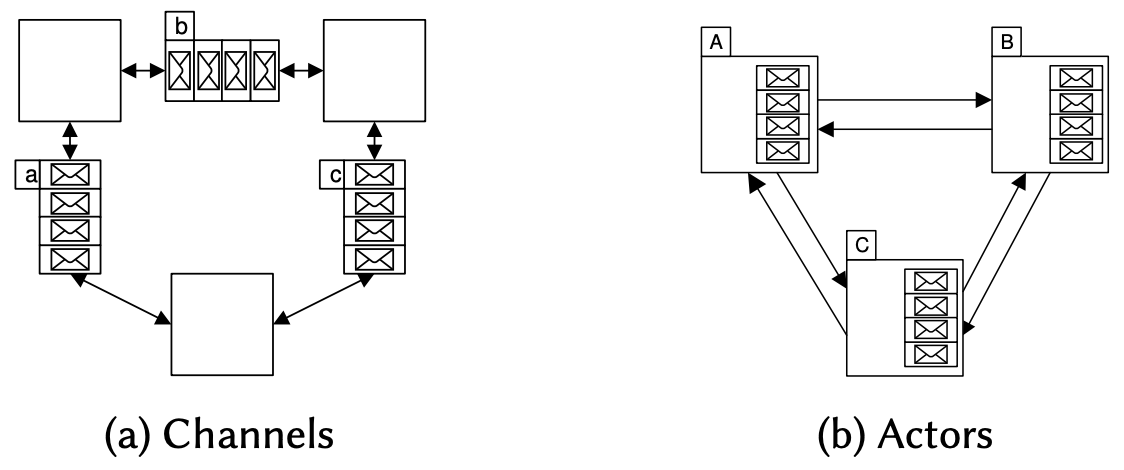
\includegraphics[width=0.7\linewidth]{images/channel_actor.png}    
    \caption{ (a) illustrates the Channels model with concurrent units communicating via message-passing channels. (b) shows the Actors model where each Actor independently processes messages from its queue. (Fowler et al. 2017)\colorbox{yellow}{referenceHere[6]}
    }
    \label{fig:channel_actor} 
\end{figure}

\subsection{Pat's Solution}
To cope with these challenges, the introduction of Actor type systems has become an important advancement. In this context, the design of the Pat language introduces a new solution based on the Actor model along with a mailbox behavioural type system for the first time in a behavioural type system at the programming language level.


\section{Mailbox}
The mailbox communication mechanism is a core concept of concurrent programming widely used in a variety of programming environments, introduced by W.S. Ford and V.C. Hamacher in 1976\colorbox{yellow}{referenceHere[4]}. It allows program components to exchange messages asynchronously, thus enabling efficient communication between processes or threads. And Erlang, as a language designed for concurrent and distributed programming, deeply integrates the mailbox communication mechanism as the cornerstone of its inter-process communication.

The Listing \ref{lst:erlangExample} is a concrete example of the application of the mailbox communication mechanism in Erlang: an asynchronous task processing model. In this model, the \textbf{empty\_task} function is a standby process that performs an asynchronous computation by receiving a message containing a Result. When the computation is complete, the Result is passed to the \textbf{queryable\_task} function. The function is in a waiting state, ready to respond to the client's query request and by sending the result of the computation back to the requester. In addition, it handles error status and returns an error if the computation request is received again. The client starts the asynchronous task through the client function, first creating a new process to run \textbf{empty\_task} through spawn, then sending computation commands and query commands to the process, and eventually receiving and printing out the results of the computation.

However, it also reveals some potential problems, such as the risk of self-deadlock. Self-deadlock occurs when a process waits for an event that will never occur, causing the process to hang permanently. In this example, if the AsyncTask process fails to receive any kind of query request after completing a computation task, possibly due to a client failure or logic error that did not send a query message, the \textbf{queryable\_task} will wait indefinitely for the query request, resulting in wasted resources and potential system performance degradation. Additionally, if the client mistakenly sends the computation command again instead of the query command, although the program is designed to return an error, this does not elegantly address the problem of receiving the computation request again in the asynchronous task completion state, and may result in unnecessary error handling and resource usage.

\lstset{style=erlangstyle}
\begin{lstlisting}[caption={Asynchronous task handling and querying implemented in Erlang}, label={lst:erlangExample}]
empty_task() ->
    receive
        { compute, Result} -> queryable_task(Result)
    end.
    
queryable_task(Result) ->
    receive
        { query, Pid } -> 
            Pid ! { reply, Result },
            queryable_task(Result); 
        { compute, _ } -> erlang:error("Task already computed") 
    end.
    
client() ->
    AsyncTask = spawn(async_task, empty_task, []),
    AsyncTask ! { compute, 2 },
    AsyncTask ! { query, self() },
    receive
        { reply, Result } ->
            io:fwrite("Task result: ~w~n", [Result])
    end.
\end{lstlisting}

\subsection{Behavioural Type System}
To solve these problems, the behavior type system provides a solution. Behavioural type system is a type system used in the field of concurrent and distributed programming to describe and manage system behaviour. This type system not only contains information about the type of data, but also extends to the description of program behaviour, such as message passing, inter-process communication patterns and protocol constraints. The core purpose of a behavioural type system is to improve the reliability and security of concurrent programs. By checking the behavioural patterns of a program at compile time, a behavioural type system ensures the correctness and stability of the program at runtime.

\subsection{Mailbox Type}
Mailbox types are an essential part of behavioral type systems, originally used in process algorithms to capture mailbox contents mainly in the form of exchanged regular expressions. Mailbox types were introduced by Ugo de'Liguoro and Luca Padovani in 2018 [3]\colorbox{yellow}{referenceHere[3]} to enhance the message-passing mechanisms of programming languages based on the role model. In the Pat language, each actor's mailbox is defined in detail through type annotations that specify not only the types of messages that the mailbox can receive, but also contain expected behavioral patterns such as the order in which messages are sent and received. This fine-grained type annotation allows developers to perform strict type checking of message passing patterns to achieve precise control of complex communication behaviors, which significantly improves the type safety of concurrent programming and effectively avoids common concurrency problems such as violation of communication protocols and deadlocks.

The following code snippet(Listing \ref{lst:patexample2}) from Pat's program demonstrates the application of mailbox types in real-world programming.This code simulates the processing of asynchronous compute and query tasks by defining \textbf{emptyTask} and \textbf{queryableTask} functions, as well as a client function. Where \textbf{emptyTask} is a mailbox for an empty task that can receive one \textcolor{red}{Compute} message and multiple \textcolor{red}{Query} messages. Once a \textcolor{red}{Compute} message is received, the mailbox will call \textbf{queryableTask}. and \textbf{queryableTask} represents a mailbox that has already received a \textcolor{red}{Compute} message, and this mailbox can only receive multiple \textcolor{red}{Query} messages. In these definitions, \textbf{guard} expressions are used to monitor the mailbox self and perform the appropriate actions based on the type of message received. This pattern not only shows how mailbox types can be used in Pat to control the sending and receiving of messages, but also how Pat can use the type system to statically check the behavior of concurrent programs to ensure communication protocol compliance and program robustness.

\lstset{style=patstyle}
\begin{lstlisting}[caption={Implementing Concurrent Program for Asynchronous Task Processing and Result Querying}, label={lst:patexample2}]
def emptyTask(self:EmptyTask):1 {
    guard self: Compute · *Query {
        receive Compute[result] from self -> 
            fullFuture(self, result)
    }
}

def queryableTask(self:Result:Int):1 {
    guard self: *Query{
        free -> ()
        receive Query[user] from self ->
            user ! Reply[Result];
            queryableTask(self,Result)
    }
}

def client():1 {
    let asyncTask = new in spawn emptyTask(asyncTask);
    let self = new in 
    asyncTask ! Compute[2];
    asyncTask ! Query[self];
    guard self: Reply[Result] from self ->
        free self;
        print(intToString(result))
}

\end{lstlisting}

\section{Implementation Strategies}

\subsection{Scheduling}
Scheduling in computing systems refers to the strategic scheduling and management of the order in which jobs are executed. This process is a high-level strategic decision making aimed at optimising processes and computational tasks in terms of time and resource allocation. In a concurrent environment, it is the responsibility of the scheduler to determine the timing of execution of each task to ensure that processor resources are used efficiently while minimising the task completion time. In distributed systems, the scheduler's responsibility extends to task allocation across different compute nodes, aiming to maximise the utilisation efficiency of each node in the network. Regardless of the type of system, the fundamental purpose of scheduling is to improve the overall throughput capacity of the system. In this framework, control flow management techniques, such as CPS and CEK, provide execution-level support and implementation mechanisms for scheduling, enabling scheduling policies to be applied more flexibly and efficiently to complex computing tasks and system architectures.

\subsection{CPS and CEK}
Continuation Passing Style (CPS) is a high-level control flow management technique that operates by explicitly passing the unexecuted portion of a program, called a "continuation". In the functional programming paradigm, this approach allows a function not to return a result directly, but to continue execution by accepting another function (i.e., a "continue") and passing it control. This style is inherently suited to implementing non-blocking and asynchronous operations, and provides a great deal of flexibility in modern programming. Although CPS elegantly handles asynchronicity and non-blocking operations, it introduces the need for concurrent multi-process control and complex communication patterns in concurrent and distributed system applications. However, CPS applications may make the code structure appear more complex and rigid, which not only challenges the readability of the programme but also increases the maintenance cost.

The Pat language, however, is dedicated to the problem of communication in concurrent and distributed systems, employing mailbox types as its core communication mechanism. In such systems, the communication process is often asynchronous, the order in which messages are delivered is uncertain, and multiple concurrent senders and receivers may be involved. In contrast to CPS, CEK-style abstract machines provide a more detailed division of programme state - Continuation, Environment and Control - through more detailed Explicit management provides a more structured and flexible framework for dealing with such complex communications. In the context of Pat language applications, where nested evaluation contexts and aliasing issues need to be considered, the CEK machine demonstrates excellent adaptability and handling capabilities, making it ideal for supporting the features of the Pat language.

\subsection{Implementing Pat in OCaml}
OCaml was chosen as the implementation language for the Pat language primarily because of its excellent capabilities in functional programming. OCaml's strong type system and pattern matching capabilities provide an intuitive and flexible approach to data processing and control flow, greatly simplifying the implementation of language features. While languages like Rust also place a high value on efficiency and safety, OCaml's unique functional programming paradigm relies much less on mutable state, and this preference for immutability effectively reduces side effects, making concurrent programming safer and easier to understand. As a result, OCaml is particularly well suited to the development of systems such as compilers and language processors that require a high degree of reliability and clear logic.


%==================================================================================================================================
\chapter{Requirements}

The purpose of this chapter is to provide a comprehensive requirements analysis of the project, including explicit functional and non-functional requirements. The detailed description of the project's core components provides clear guidance for the design and implementation of the project, ensuring that the final product will meet the intended quality standards and performance metrics.

\section{Functional Requirements}
In terms of functional requirements, we focus on the core functions that must be implemented by the interpreter, including syntax parsing, program state control, task scheduling, and memory management, to ensure the basic operation and execution efficiency of the interpreter.

\subsection{Must Have}
\textbf{Grammar parsing capability}: Must be able to accurately parse all the syntactic structures of the Pat language, including but not limited to variable declarations, control flow statements (e.g., if-else, switch), as well as support for basic data types (integers, strings).

\textbf{Mailbox processing}: Realize the creation of mailboxes, message insertion, storage, retrieval and release functions.

\textbf{Program state control}: Adopts CEK machine to achieve precise control of the execution state of the Pat program to ensure the correct execution of program logic.

\textbf{Task Scheduling}: Implements a round-robin-based task scheduling mechanism to achieve fair task scheduling and support parallel task creation and execution.

\textbf{Memory management}: Integrate Garbage Collection mechanism to effectively manage memory usage and optimize resource utilization.

\subsection{Should Have}
\textbf{Execution flow printing}: In debug mode to provide the execution of step-by-step printing to assist developers to debug and understand the program execution process.

\textbf{Error Handling Mechanism}: Design and implement a well-defined error handling mechanism to effectively manage exceptions and runtime errors.

\subsection{Could Have}
\textbf{Garbage collection optimization}: Research and implement optimized garbage collection mechanism to reduce the impact of execution time and improve execution efficiency.

\textbf{Communication system enhancement}: Enhance the mailbox communication system to improve the efficiency and reliability of message delivery.

\subsection{Won't Have}
\textbf{Scheduling Algorithm Research}: Does not delve into other scheduling algorithms that might replace the polled scheduling approach such as EIO that has the capability of parallel IO operations. in order to focus on optimization of the current implementation.

\section{Non-Functional Requirements}
Non-functional requirements relate to the usability, and cross-platform compatibility of the interpreter to ensure that the interpreter not only meets the requirements in terms of functionality, but also provides a good user experience during use.

\subsection{Must Have}
\textbf{Cross-platform compatibility}: The interpreter should be able to run seamlessly on major operating systems including Windows, Linux, macOS to ensure wide availability.

\subsection{Should Have}
\textbf{Ease of use}: Design the interpreter to be friendly to novice users so that users can get started quickly.

\subsection{Won't Have}
\textbf{IDE Integration}: Plug-in support for popular IDEs (e.g. VS Code, IntelliJ) including syntax highlighting, code auto-completion, and quick jumps to definitions is not provided at this stage.

\textbf{Debugging tools integration}: Not integrated debugging tools , including the lack of support for breakpoint settings , single-step execution and variable status view function .


%==================================================================================================================================
\chapter{Design}

\section{Principles of CEK-style Machine}

\subsection{$\lambda$-Calculus}
Before delving into the implementation and optimization of CEK machines, it is crucial to understand the underlying concepts and principles of $\lambda$-Calculus, a formal system for representing the logic of a computational process or mathematical function, introduced by mathematician Alonzo Church in the 1930s\colorbox{yellow}{referenceHere}, which is one of the core foundations of modern computer science. The system focuses on the process of binding and substitution of variables and serves as a generalized model of computation, equivalent to a Turing machine, that exhibits the fundamentals of the theory of computation.

\begin{figure}[h]
    \centering
    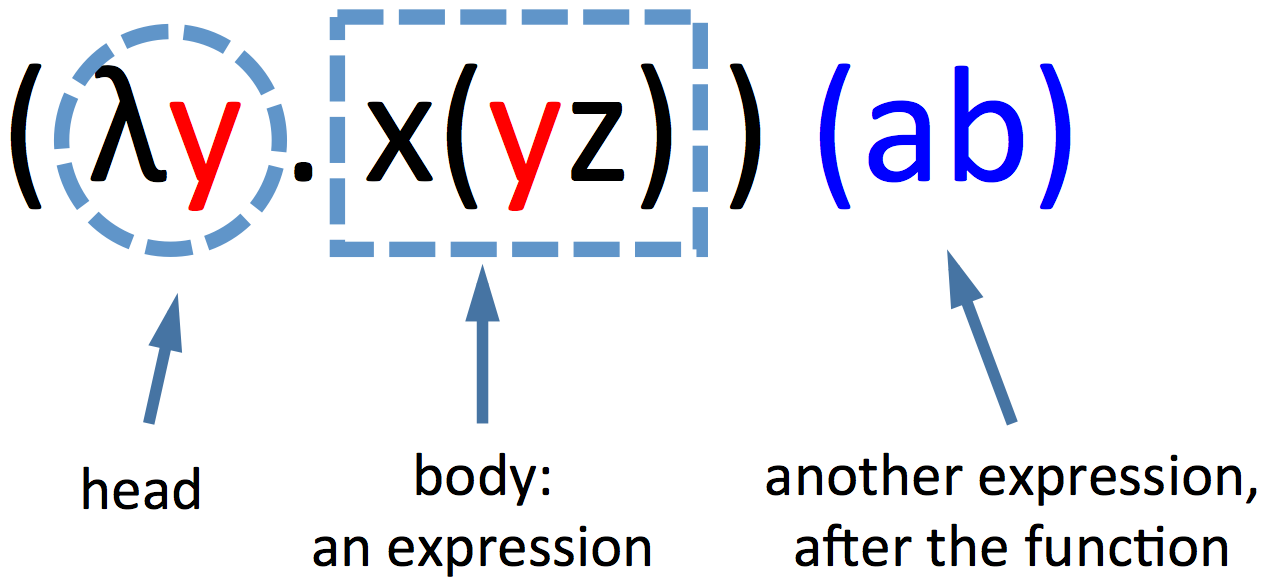
\includegraphics[width=0.35\linewidth]{dissertation/images/lambda1.png}    
    \caption{Illustration of $\lambda$-Calculus expression, showcasing the head of the expression marked in red, the body of the expression in dashed blue, and another expression following the function in solid blue.\colorbox{yellow}{referenceHere}}
    \label{fig:lambda} 
\end{figure}

In the $\lambda$-Calculus system, all functions are defined anonymously, and their definition and application are accomplished uniquely through $\lambda$-abstraction. $\lambda$-expressions essentially define a function, which is realized by binding variables and expressing the expression inside the function body. The application of the function then simply places the actual arguments after the function name, without the need to separate them with parentheses or commas(Figure \ref{fig:lambda}). For example, Consider the $\lambda$-expression for a function that adds two numbers:
\[
\lambda x.\lambda y.x+y
\]
This expression is made up of two lambda abstractions:
\begin{itemize}
    \item $\lambda x$ which creates a function that takes an argument $x$
    \item $\lambda y$ which creates a function that takes an argument $y$
\end{itemize}
When this function is applied to two numerical arguments, such as 3 and 2, the operation proceeds as follows:
\begin{align*}
\text{Apply the first number: } & (\lambda x.\lambda y.x+y)3 \rightarrow \lambda y.3+y \\
\text{Apply the second number: } & (\lambda y.3+y)2 \rightarrow 3+2 \\
\text{Evaluate the addition: } & 3+2 \rightarrow 5
\end{align*}
Hence, the application of the lambda function \(\lambda x.\lambda y.x+y\) to the arguments 3 and 2 yields the result 5, which demonstrates basic function creation and application in lambda Calculus.

\subsection{Traditional CEK Machine}

The CEK machine, developed by Matthias Felleisen and Dan Friedman (1986)\colorbox{yellow}{referenceHere}, is a machine for $\lambda$-Calculus that is particularly well suited for describing and enforcing the semantics of functional programming languages. This machine, with its realism and abstraction, provides a framework to show how computers can efficiently execute programs. The basic CEK machine is based on a ternary configuration of the form $⟨C\:|\:E\:|\:K⟩$. where
\begin{itemize}
    \item $\textbf{C}$ for Control, the expression currently being evaluated;
    \item $\textbf{E}$ for Environment, binding free variables;
    \item $\textbf{K}$ for Continuation, which guides the action taken by the machine after completing the evaluation of the current term $C$.
\end{itemize}
Let us consider an expression "let $x$ = 3 in $x$ + 2". On this occasion we will execute it using the CEK machine:
\begin{align*}
& \left\{C: \textcolor{red}{\text{let } x = 3 \text{ in } x + 2}, E: \{\}, K: \text{empty}\right\} \\
\rightarrow & \left\{C: \textcolor{red}{3}, E: \{\}, K: \textcolor{red}{\text{let } x = [] \text{ in } x + 2}\right\} \\
\rightarrow & \left\{C: \textcolor{red}{x + 2}, E: \{\textcolor{blue}{x: 3}\}, K: \text{empty}\right\} \\
\rightarrow & \left\{C: \textcolor{red}{5}, E: \{\textcolor{blue}{x: 3}\}, K: \text{empty}\right\}
\end{align*}
In the initial phase, the CEK machine sets the control section to the full expression $\color{red}{\text{let } x = 3 \text{ in } x + 2}$. At this point, the environment is empty, indicating that no variable binding has been evaluated yet, and the continue section is also empty, indicating that no further computations are waiting to be evaluated. Next, the CEK machine recognizes the variable binding action in the $\color{red}{\text{let}}$ statement and begins to add the variable $\color{red}{x}$ to the environment in preparation for its association with the value $\color{red}{3}$. During this process, the control section is updated to $\color{red}{3}$, the environment is updated accordingly to contain the mapping $\color{blue}{\{x: 3\}}$, and the expression $\color{red}{x + 2}$ is placed in the continue section, waiting for a subsequent computation. When evaluating the computation of $\color{red}{x + 2}$, the CEK machine looks up and replaces the variable $\color{red}{x}$ with $\color{red}{3}$ in the environment, and then evaluates an addition operation to obtain the final result $\color{red}{5}$.

\subsection{Generalized CEK Machine}
In the design of the Pat language, reference was made to Daniel Hillerstrom and Sam Lindley's work\colorbox{yellow}{referenceHere} on the generalization of the traditional CEK machine. This generalization process is particularly important for the Pat language because the traditional CEK machine was designed primarily for simple functional programming languages, which are overwhelmed when dealing with complex control flow and state management---especially algebraic effects. In the generalized CEK machine(Figure 4.2), the configuration takes the form of $\langle \boldsymbol{M}\: |\: \boldsymbol{\gamma} \:| \:\boldsymbol{\Sigma} \rangle$, where $\boldsymbol{M}$ represents the current term to be computed, which is equivalent to the control (C) part in the original CEK machine. $\boldsymbol{\gamma}$ represents the current environment, inherited from the environment (E) part in the original machine, which is in charge of binding the variables to the corresponding values. $\boldsymbol{\Sigma}$, on the other hand, represents the continuation part, which, unlike the continuation (K) of a single instruction or state in the original machine, consists of a series of continuation frames $[\boldsymbol{\delta}_1, \ldots , \boldsymbol{\delta}_n]$, each frame $\boldsymbol{\delta} = (\boldsymbol{\chi}, \boldsymbol{\gamma}, \boldsymbol{M})$ representing a pure continuation within a particular processor closure. Here $\boldsymbol{\chi}$ denotes the processor closure (handler closure), $\boldsymbol{\gamma}$ maintains its role as an environment for mapping variables to their values, and $\boldsymbol{M}$ represents the current computational term or expression being evaluated. 
\begin{align*}
\text{ Configurations}\;\; & C ::= \langle M \, | \, \gamma \, | \, \Sigma \rangle \\
\text{Environment}\;\; & \gamma ::= \cdot \, | \, \gamma, x \mapsto V \\
\text{ Frame stack}\;\; & \Sigma ::= \cdot \, | \, \sigma \circ \Sigma \\
\text{Frame}\;\; & \sigma ::= \langle \chi, \gamma, M \rangle \\
\text{Value}\;\; & v ::= \gamma(v) 
\end{align*}
\begin{center}
\textit{\textbf{Figure 4.2:} CEK Syntax}
\end{center}
\vspace{10pt}
With this design, even though \textbf{Yield} functionality is not usually provided directly in functional programming paradigms, the model effectively implements yield-like behavior. This is particularly important for thread scheduling in Pat. In a concurrent environment, \textbf{Yield} allows a thread to actively release processor resources, thus allowing the scheduler to allocate resources to other threads or tasks. The continuation part of the generalized CEK machine $\boldsymbol{\Sigma}$ provides the basis for implementing this operation. Each continue frame can be thought of as a pause point that contains all the information needed to resume execution, similar to the pause and resume mechanism of the yield operation.

Let us execute the expression again: let x = 3 in x + 2, this time with a generalized CEK machine:
\begin{align*}
& (M: \textcolor{red}{\text{let } \ x\ =\ 3\ \text{in } \ x\ +\ 2}, \gamma: \{\}, \Sigma: \text{empty}) \\
\rightarrow & (M: \textcolor{red}{3}, \gamma': \{\}, \Sigma: \langle M: \textcolor{red}{x}, \gamma: \{\}, (\textcolor{red}{x+2})\rangle \cdot \Sigma) \\
\rightarrow & (M: \textcolor{red}{x\ +\ 2}, \gamma: \{ \textcolor{blue}{x} \mapsto \textcolor{blue}{3}\}, \Sigma: \text{empty}) \\
\rightarrow & (M: \textcolor{red}{\text{\textlbrackdbl} x \text{\textrbrackdbl}}_{\gamma} + \textcolor{red}{2}, \gamma: \{ \textcolor{blue}{x} \mapsto \textcolor{blue}{3}\}, \Sigma: \text{empty}) \\
\rightarrow & (M: \textcolor{red}{3\ +\ 2}, \gamma: \{ \textcolor{blue}{x} \mapsto \textcolor{blue}{3}\}, \Sigma: \text{empty}) \\
\rightarrow & (M: \textcolor{red}{5}, \gamma: \{ \textcolor{blue}{x} \mapsto \textcolor{blue}{3}\}, \Sigma: \text{empty})
\end{align*}

Included in its initial state are the entire expression as the machine state \(M\), an empty environment \(\gamma\) indicating that there are no variables bound, and an empty stack \(\Sigma\) implying that there are currently no computations to be executed. This setup is similar in nature to a traditional CEK machine. However, as the evaluation process unfolds, the machine state is first updated to {\color{red}3}, signaling that the variable $\color{red}x$ is about to be bound to it, and simultaneously pushing the expression $\color{red}x + 2$ onto the stack, awaiting further computation. The role of the stack in this step is to hold the current computational context, including variables and environment, which is very different from the traditional CEK machine that simply puts the expression to be continued into the "continue" section.

Subsequently, when the machine state changes to $\color{red}x + 2$, the environment is updated to $\color{blue}x \rightarrow 3$, which shows that $\color{red}x$ has been successfully bound to {\color{red}3}. At this point, the stack is cleared, indicating that the system is ready to execute the expression. Next, the machine state expression $\color{red}\text{\textlbrackdbl} V \text{\textrbrackdbl}_{\gamma} + 2$ is computed by looking up in the environment and replacing $\color{red}x$ with {\color{red}3}, which in turn is transformed to {\color{red}3} + {\color{red}2}. Eventually, the machine status is updated to {\color{red}5}, signaling that the computation has been successfully completed. This example not only shows how the generalized CEK machine handles complex expressions and variable bindings but also highlights the importance of the stack in preserving execution context.

\begin{align*}
\text{E-LET} & \quad \llparenthesis \ \textbf{let} \ x: T = M \textbf{ in } N, \Sigma \ \rrparenthesis \rightarrow \llparenthesis \  M, \langle x, N \rangle \cdot \Sigma \ \rrparenthesis \\
\text{E-RETURN} & \quad \llparenthesis \ V, \langle x, M\rangle \cdot \Sigma \ \rrparenthesis \rightarrow \llparenthesis \ M\{V/x\}, \Sigma \ \rrparenthesis \\
\text{E-APP} & \quad \llparenthesis \ f(\overrightarrow{V}), \Sigma \ \rrparenthesis \rightarrow \llparenthesis \ M\{\overrightarrow{V}/\overrightarrow{x}\}, \Sigma \ \rrparenthesis \quad \text{if } \Roman{P}(f) = \text{def } f(\overrightarrow{x} : A) : B \{ M \} \\
\text{E-NEW} & \quad \llparenthesis \ \texttt{new}, \Sigma \ \rrparenthesis \rightarrow \llparenthesis \  va, (a, \Sigma) \ \rrparenthesis \quad (a \text{ is fresh}) \\
\text{E-SEND} & \quad \llparenthesis \ a!m\overrightarrow{V}, \Sigma \ \rrparenthesis \rightarrow \llparenthesis \ (), \Sigma \parallel a \leftarrow m\overrightarrow{V} \ \rrparenthesis \\
\text{E-SPAWN} & \quad \llparenthesis \ \texttt{spawn } M, \Sigma\ \rrparenthesis \rightarrow \llparenthesis \  (), \Sigma \parallel (M, \varepsilon)\rrparenthesis \\
\text{E-FREE} & \quad \llparenthesis \  va)((\texttt{guard } a: E \{ G[\texttt{free } h \rightarrow M]\}), \Sigma\ \rrparenthesis \rightarrow \llparenthesis \ M, \Sigma \ \rrparenthesis
\end{align*}


\begin{equation}
  \llbracket     1 \rrbracket       \quad
  \llparenthesis 2 \rrparenthesis   \quad
  \llceil        3 \rrceil          \quad
  \llfloor       4 \rrfloor         \quad
\end{equation}


\section{Pat Scheduling}
The generalized CEK machine provides an execution-level support and implementation framework for the scheduling mechanism of the Pat language.Pat chooses the Round-Robin scheduling mechanism as a fair scheduling strategy, which centers on ensuring that all threads are given an equal amount of processor time, thus preventing any thread from occupying CPU resources for a long period of time. In Pat, this mechanism is improved by changing the time to steps to ensure that all threads get the same number of evaluation steps. This strategy effectively prevents threads from waiting indefinitely after a message is delivered. Once the evaluation steps of a thread reaches the preset upper limit, the system will automatically switch to the next thread in the queue, which ensures the timeliness of message processing between threads and avoids the problem of message backlog.

Figure 4.3 shows a simplified example of the Pat scheduling mechanism, where the active steps of each process are represented by the length of the color slice, and different colored slice are used to distinguish between processes. In this model, the maximum value of the step slice is set to 2, which means that after any process executes two steps, the scheduler will force it to move to the next process. The diagram clearly shows the state of the four processes (P1 to P4) during the execution steps. Process P1 reaches the maximum step slice limit after two steps of execution. Process P2 still has one step left to complete after the second step, at which point the scheduling mechanism interrupts P2 and switches to the execution of P3. After P3 completes, the system returns to complete the remaining steps of P2. Finally, P4 is executed similarly to P1. This allocation model ensures that the processes are executed sequentially in a fixed number of steps, reflecting the fairness of the rotation scheduling strategy and ensuring that no process will monopolize the processor resources for a long time.

\begin{center}
\begin{tabular}{c|*{9}{p{0.5cm}}}
\rowcolor{white}
\multicolumn{1}{c|}{Process\textbackslash Step} & \multicolumn{1}{c}{1} &\multicolumn{1}{c}{2} &\multicolumn{1}{c}{3} &\multicolumn{1}{c}{4} &\multicolumn{1}{c}{5} &\multicolumn{1}{c}{6} &\multicolumn{1}{c}{7} &\multicolumn{1}{c}{8} &\multicolumn{1}{c}{9} \\ \hline
P1 & \cellcolor{blue!25} & \cellcolor{blue!25} & & & & & & & \\
P2 & & & \cellcolor{red!25} & \cellcolor{red!25} & & & \cellcolor{red!25} & & \\
P3 & & & & &\cellcolor{green!25} & \cellcolor{green!25} & & & \\
P4 & & & & & & & & \cellcolor{yellow!25} & \cellcolor{yellow!25} \\
\end{tabular} \\
\textit{\textbf{Figure 4.3:} Pat's Round-Robin Scheduling}
\end{center}



















%==================================================================================================================================
\chapter{Implementation}
What did you do to implement this idea, and what technical achievements did you make?
\section{Guidance}
You can't talk about everything. Cover the high level first, then cover important, relevant or impressive details.



\section{General points}

These points apply to the whole dissertation, not just this chapter.





%==================================================================================================================================
\chapter{Evaluation} 
In this research, we comprehensively evaluated the effectiveness of the Pat language runtime interpreter, employing methods such as correctness testing and micro-benchmarking, aiming to accurately quantify its performance metrics. Correctness testing ensured that the Pat language executed as expected when processing different example files, verifying the correctness of the language design and runtime. The efficiency of the interpreter in performing computationally intensive tasks was evaluated through careful measurements of the runtime of specific algorithmic tasks (e.g., computing Fibonacci series), and these tests focused on evaluating the performance of the Pat language under real-world running conditions. The tests were performed on a computer equipped with an M2 Pro chip and 16 GB of RAM, with the operating system MacOS 14.3, using the OCaml version 5.1.0 environment, and the time calculations, which included all parts of the type checking and the interpreter, were repeated about 100 times, thus ensuring the accuracy and reliability of the results.

\section{Concurrent Reduction}

\subsection{Functional Reduction}
In performing a series of fundamental tests on the Pat language, we aim to verify whether the Pat language is able to accurately execute basic programming constructs and how well it performs in different programming scenarios. These tests help to evaluate whether the runtime environment of the Pat language can meet the needs of concurrent and distributed systems programming, and whether it can correctly handle various programming tasks according to its design specifications.

Specific tests performed include basic arithmetic tests, operator precedence, logical operation tests, anonymous functions, local variables and function bindings, empty interfaces and linear functions, and pattern matching. The results of the tests show (Table \ref{tab:Fundamental_results}) that all tests were successfully completed as expected and no runtime errors were found. This result proves that the underlying functionality of the Pat language matches the design specifications and is capable of handling a wide range of programming tasks.

\begin{table}[ht]
\centering
\renewcommand{\arraystretch}{1.1}
\resizebox{\textwidth}{!}{%
\begin{tabular}{l l c c}
\toprule
\textbf{Name}  & \textbf{Description}   & \textbf{Exp.} & \textbf{Act.}  \\
\midrule
Arithmetic I  & Basic arithmetic check & True & True \\
Arithmetic II  & Operator precedence checks arithmetic order & True & True \\
Arithmetic III & Logic \& arithmetic test combines operations  & False & False \\
Anonymous Function & Function returns input integer value & 5 & 5 \\
Local Binding & 
Local binding and function definition & 10 & 10 \\
Nested Binding & Nested function returns double input value & 10 & 10 \\
Memory Management & Interface declaration and memory deallocation & - & - \\
Pattern Matching (Left) & Handles union type and printing & 5 & 5 \\
Pattern Matching (Comprehensive) & Evaluates type inference & 5 & 5 \\
\bottomrule \\
\end{tabular}%
}
\caption{Basic Correct Test Results}
\label{tab:Fundamental_results}
\end{table}




\subsection{Concurrency Reduction}
After the basic correct tests were completed, we further tested the correctness of six advanced concurrency models for the Pat language, based on the original mailbox algorithmic model with ideas taken from the research of de'Liguoro and Padovani (2018)\colorbox{yellow}{referenceHere}. The specific test implementations refer to the research of Fowler et al. (2023)\colorbox{yellow}{referenceHere}. These test cases cover everything from concurrent lock, future variable handling, and account concurrent transactions, account concurrent transactions via future variables, master-worker parallel networks, and session-type communication actor models using a single arbiter.

First, we simulate concurrent locks to verify the efficiency and reliability of the Pat language in handling mutually exclusive operations. In addition, we evaluated the performance of the Pat language in handling one-time write and multiple read operations by testing the "Future" variable. Then, by simulating debit/credit instruction exchanges between concurrent accounts, we further validate the accuracy and efficiency of the Pat language in complex concurrency scenarios. In order to explore the application of Pat in asynchronous programming model, we also test the debit/credit commands of accounts implemented by "Future". In addition, we evaluate the performance of the Pat language in a distributed computing environment by constructing a parallel network of master-worker jobs. Finally, we explore the ability of the Pat language to implement complex communication protocols through a session-type communication actor model, which involves the use of a single arbiter to coordinate communication behavior.

All tests show that the Pat language is able to successfully handle these high-level concurrent and distributed programming tasks, demonstrating alignment between expected and actual outcomes(Table \ref{Concurrency_result}). The test results not only validate the performance of the Pat language in different programming scenarios, but also demonstrate its power in handling concurrent and distributed system programming requirements. The average response times ranged from 45.8 ms for the concurrent model to 102.9 ms for the session type model, further proving that the Pat language is able to provide a high degree of functionality and reliability while ensuring performance.
\begin{table}[ht]
\centering
\renewcommand{\arraystretch}{1.1}
\resizebox{\textwidth}{!}{%
\begin{tabular}{l l c c}
\toprule
\textbf{Name}       & \textbf{Description}   & \textbf{Exp.}  & \textbf{Act.}\\
\midrule
Lock   & Concurrent lock modelling mutual exclusion       & 12 & 12  \\
Future  & Future variable that is written to once and read multiple times & 55         & 55          \\
Account             & Concurrent accounts exchanging debit and credit instructions  & - & -                 \\
Account Future & Concurrent accounts where debit instructions are effected via futures  & INFO.. & INFO..                  \\
Master-Worker       & Master-worker parallel network            & 55385 & 55385                  \\
Session Types       & Session-typed communicating actors using one arbiter   & 6 & 6                 \\
\bottomrule \\
\end{tabular}%
}
\caption{Advanced Concurrency Model Correct Test Results \colorbox{yellow}{referenceHere}}
\label{Concurrency_result}
\end{table}


\section{Micro-Benchmark Test}

Based on the correctness tests, we designed and implemented a series of benchmark tests aimed at evaluating the performance of the Pat language's runtime interpreter under different concurrent programming patterns. These tests cover a wide range of concurrent programming scenarios including master-worker (e.g., KFork, Fibonacci, Log Map), client-server (e.g., Ping Pong, Counter), and peer-to-peer (e.g., Big), and involve common network topologies such as Star (e.g. Philosopher, Smokers, Transaction) and Ring (e.g. Thread Ring) \colorbox{yellow}{referenceHere}. Each test is designed to evaluate the execution efficiency of the Pat language under a particular concurrency model.

The purpose of these benchmarks is to establish an initial performance baseline for the Pat language and to demonstrate that it can effectively handle multiple concurrency models. Given that the Pat language is the first programming language to integrate mailbox typing, we do not use the results of these tests for direct comparisons with existing functional languages on the market. Instead, our goal is to demonstrate the controlled operation of the Pat language by showing how it can stably execute multiple concurrency patterns based on a design and implementation that incorporates the concept of mailbox types.

Through this series of benchmark tests, we observe the performance of the Pat language under different concurrency models (table \ref{Savina}). For example, the Ping Pong test evaluates the message processing speed by simulating the bidirectional delivery of messages; the Thread Ring test measures the message delivery latency by passing tokens in a ring network; and the Fibonacci test demonstrates the efficiency of the Pat language in handling recursive concurrency tasks. In the K-Fork test, we made the necessary adjustments. In the original setup, the central actor distributes a large number of requests to the workers, resulting in a huge amount of data, which affects the execution efficiency of the test and the accuracy of the results. In order to more accurately evaluate the performance of the Pat language in handling concurrent tasks, we reduced the number of workers to ensure that the test results can more truly reflect the actual performance of the language. Note that in the Smokers test, this design caused a significant increase in test execution time due to the introduction of a randomized sleep function.

\begin{table}[ht]
\centering
\renewcommand{\arraystretch}{1.1}
\resizebox{\textwidth}{!}{%
\begin{tabular}{l l c}
\toprule
\textbf{Name} & \textbf{Description} & \textbf{Avg Time (ms)} \\
\midrule
Ping Pong & Process pair exchanging \( k \) ping and pong messages & 54.5 \\
Thread Ring & Ring network where actors cyclically relay one token with counter \( k \) & 541.5 \\
Counter & One actor sending messages to a second that sums the count & 45.5 \\
K-Fork & Fork-join pattern where a central actor delegates \( k \) requests to workers & 298.9 \\
Fibonacci & Fibonacci server delegating terms \( (k - 1) \) and \( (k - 2) \) to parallel actors & 56.7 \\
Fib\_pairs & Fibonacci actors recursively resolving and returning terms independently & 55.1 \\
Big & Peer-to-peer network where actors exchange \( k \) messages & 265.8 \\
Philosopher & Dining philosophers problem & 111.9 \\
Smokers & Centralised network where one arbiter allocates \( k \) messages to actors & 5578.4 \\
Log Map & Computes the term \( xx + 1 = r \cdot xx \cdot (1 - xx) \) by delegating to parallel actors & 97.9 \\
\bottomrule \\
\end{tabular}
}
\caption{Part List of Savina Benchmarks. \colorbox{yellow}{referenceHere}}
\label{Savina}
\end{table}

The composite graph(Figure \ref{fig:benchmark}) presents the execution time test results of four different program fragments in Pat language with different K values. From top to bottom, left to right, they are Fibonacci computation time, Ping Pong performance analysis, bank request-response chain performance, and log-mapping simulation performance. It can be observed that the execution time curves for both sequential and concurrent execution are quite close to each other, indicating that no significant additional overhead is introduced in concurrent execution.

For the execution time fluctuations observed in the two graphs below, this may be due to the small time scale used for testing, which makes even minor execution variations appear as large fluctuations in the graphs. Such fluctuations may arise from system scheduling, memory cache efficiency, and other non-deterministic factors in the test environment. These results show the stability of the Pat language in handling different types of concurrent tasks and its potential to maintain low overhead for concurrent operations.

\begin{figure}
    \centering
    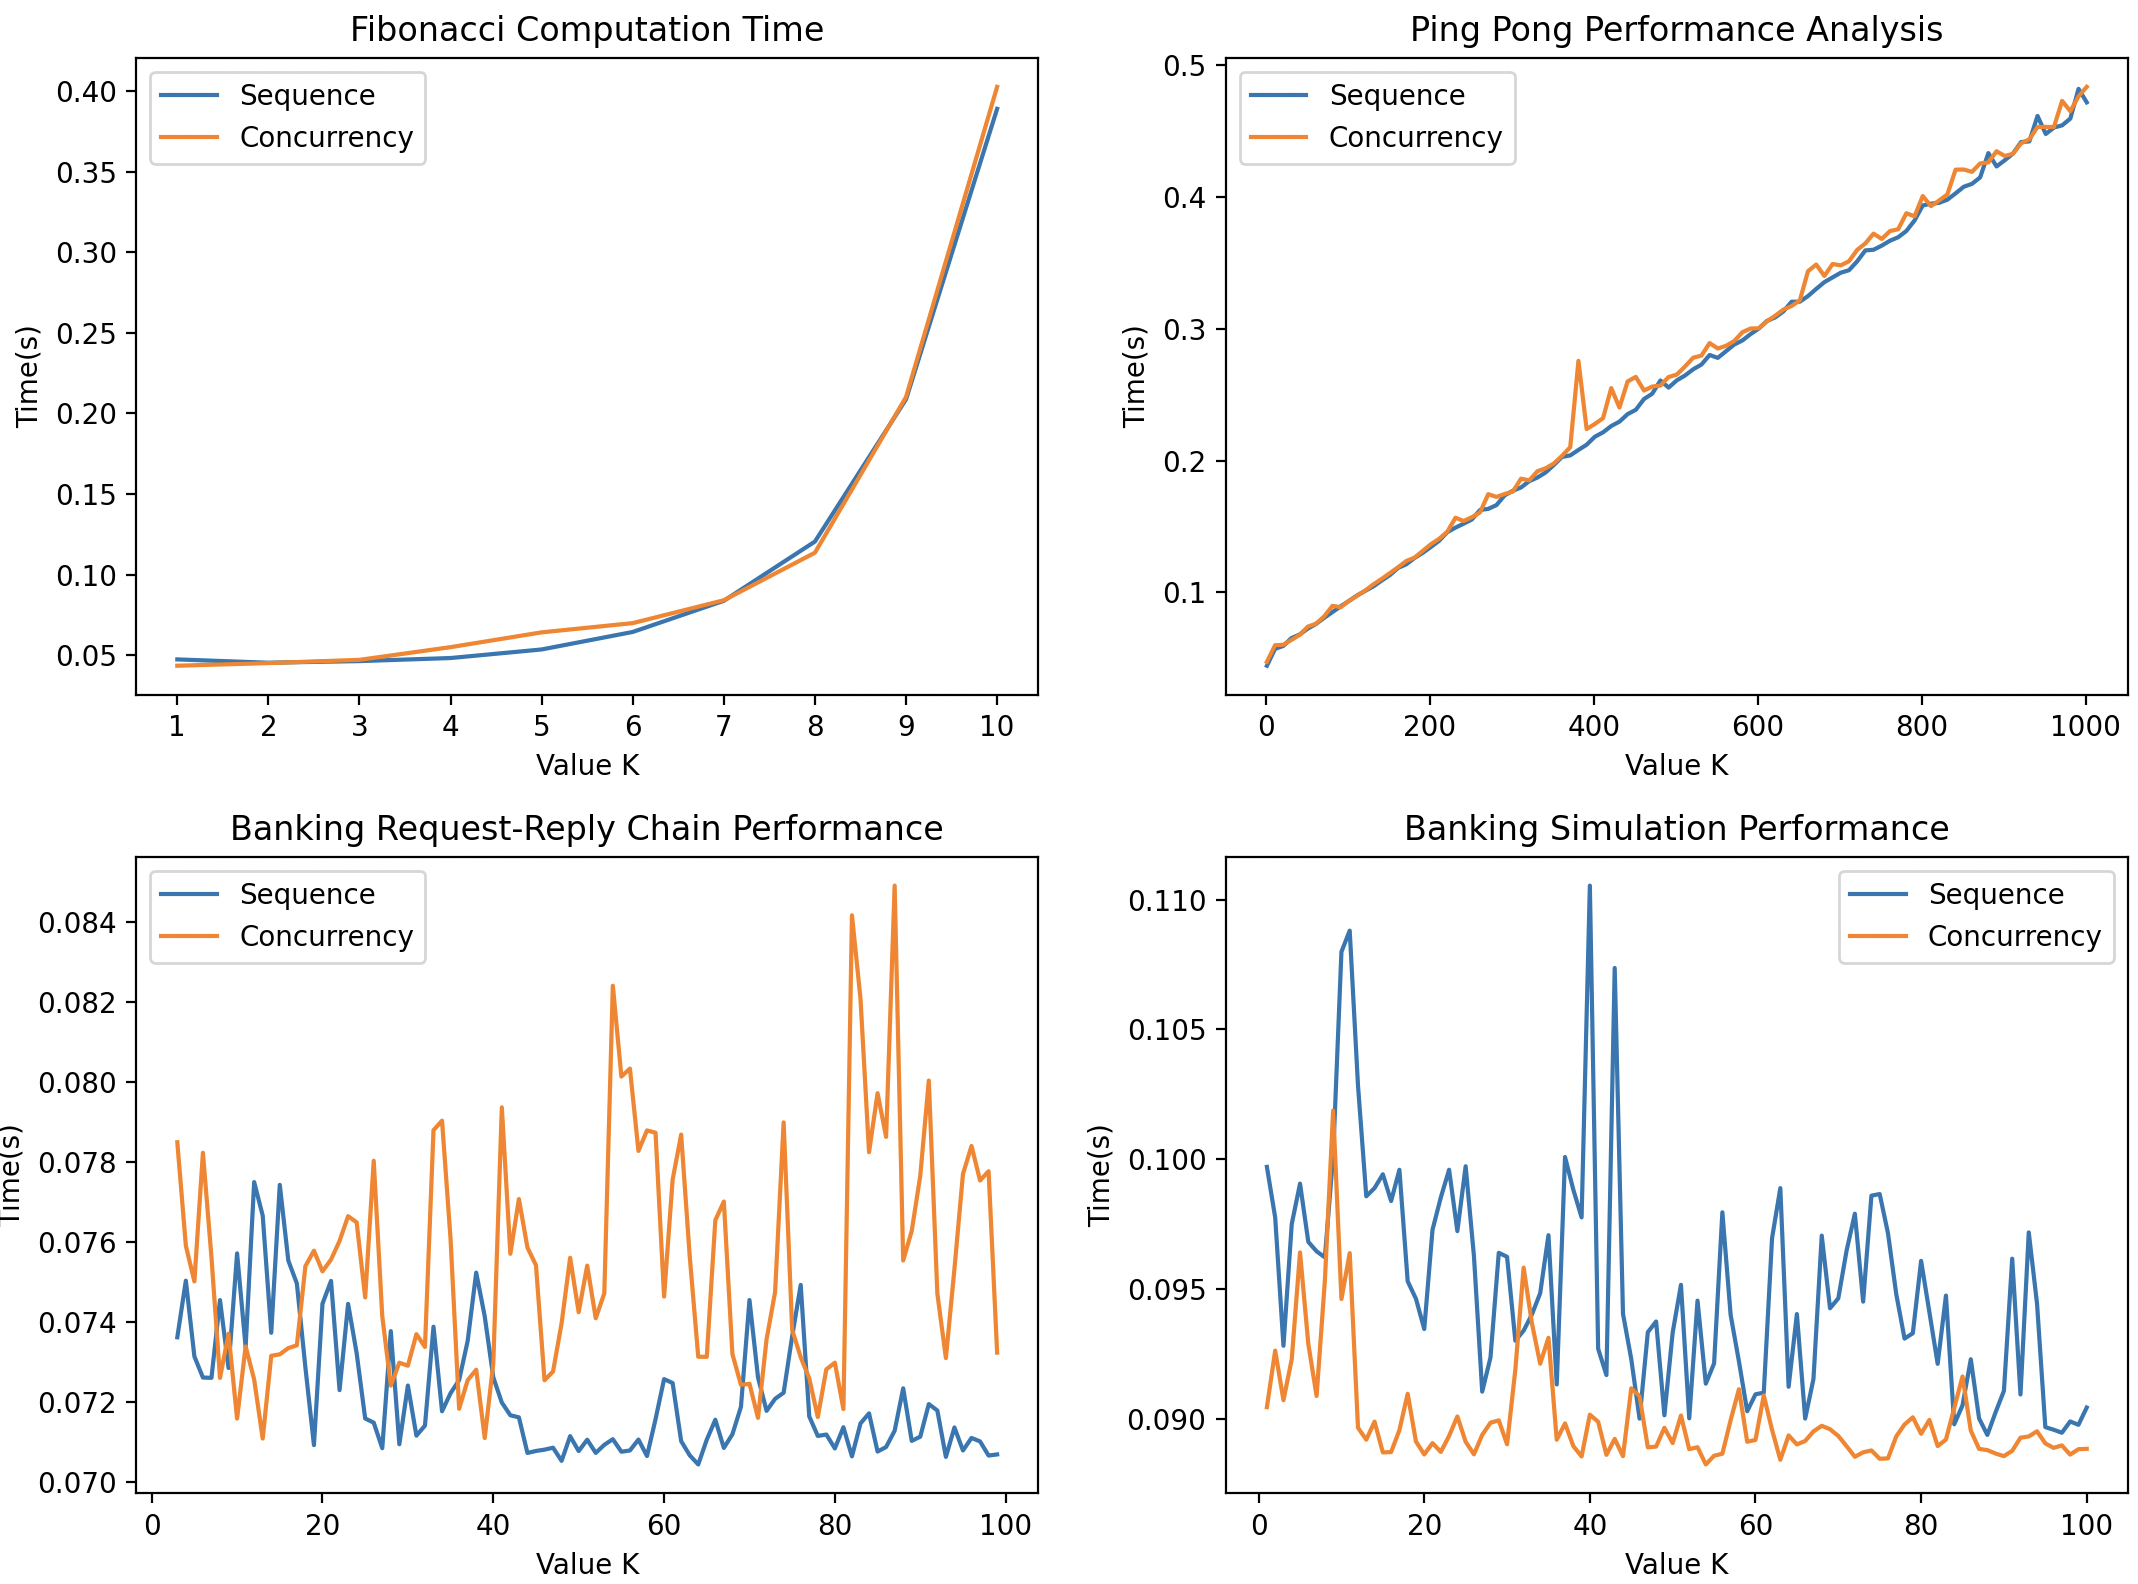
\includegraphics[width=0.9\linewidth]{dissertation/images/benchmark.png}    
    \caption{ 
    Comparative Execution Times of Sequential and Concurrent Code Snippets in Pat Language at Various K Values
    }
    \label{fig:benchmark} 
\end{figure}

In summary, these benchmark tests provide us with a comprehensive evaluation framework to scrutinize the performance of the Pat language in the area of concurrent programming. The unique advantages of the Pat language in handling complex concurrent tasks are demonstrated. This research provides important references and insights for the future development of functional language design and concurrent programming patterns for mailbox types.

\section{Reflection}
In the reflection section, the discussion of the research on garbage collection optimization and scheduling algorithms reveals two key areas in our research and development process, as well as pointing to potential directions for future work.

\subsection{Garbage Collection Optimization}

For garbage collection optimization section, we currently employ a mechanism that similarly combines a simple Mark-Sweep algorithm and a Reference Counting method. This approach provides our system with basic memory management capabilities. Although this combined strategy works effectively in many cases, we also recognize its limitations when dealing with branching statements such as if/switch, and complex programming constructs such as recursion. Especially in recursive calls and complex control flow structures, the simple reference counting method may not be able to accurately identify all garbage objects, resulting in memory not being reclaimed in a timely manner, thus affecting the execution efficiency and stability of the system.

Therefore, if we have more time, we plan to explore and implement a more in-depth reference counting mechanism. This advanced reference counting method will be optimized especially for branching structures and recursive calls in programming. For example, by introducing a branch-sensitive reference counting update mechanism, we can more accurately track the lifecycle of an object at runtime, and thus more intelligently manage the reference counting of objects in different branching paths. In addition, for the optimization of recursive structures, we can consider introducing tail recursion optimization or specific recursive pattern recognition to reduce unnecessary memory occupation and improve the accuracy of reference counting.

This in-depth reference counting strategy not only improves the efficiency of garbage collection and reduces the cases of incorrectly reclaiming or retaining objects, but also optimizes the memory usage while ensuring the performance of the system. By researching and implementing these advanced features, we expect to further mitigate the impact of garbage collection on program execution and improve the execution efficiency and responsiveness of the entire system.

\subsection{Advanced Scheduling Algorithms}

Regarding the research on scheduling algorithms, our current implementation employs the Round-Robin scheduling approach, which is a simple and straightforward scheduling strategy. However, we also recognize that other framework, such as the EIO scheduling, which is capable of supporting parallel IO operations, may provide better performance and efficiency(Figure \ref{lst:eio}).The introduction of EIO not only takes advantage of the high-performance IO operation features provided by modern operating systems, such as Linux's io\_uring, but also allows concurrent code to be written in a much more concise and efficient manner through a direct style of IO stacking. This approach does a lot more than just reduce heap allocation and increase speed, it also makes concurrent code written in the same style as non-concurrent code, which greatly improves the readability and maintainability of the code.

Within the time constraints of the project, we did not explore these alternatives in depth. Had we had more time, we would have compared the performance of different algorithms under multiple loads and scenarios, and we could have determined the scheduling strategy that best suited our system. In addition, research on how to combine multiple scheduling strategies in order to dynamically select the scheduling algorithm that best suits the current execution environment and task characteristics will also be a focus of our attention.

\noindent\begin{minipage}{\linewidth}
\lstset{style=ocamlstyle}
\begin{lstlisting}[caption={Example of running two threads of execution concurrently using Eio.Fiber \colorbox{yellow}{referenceHere}}, label={lst:eio}]
let main _env =
  Fiber.both
    (fun () -> for x = 1 to 3 do traceln "x = %d" x; Fiber.yield () done)
    (fun () -> for y = 1 to 3 do traceln "y = %d" y; Fiber.yield () done);;
\end{lstlisting}
\end{minipage}


%==================================================================================================================================
\chapter{Conclusion}    
Summarise the whole project for a lazy reader who didn't read the rest (e.g. a prize-awarding committee).
\section{Guidance}
\begin{itemize}
    \item
        Summarise briefly and fairly.
    \item
        You should be addressing the general problem you introduced in the
        Introduction.        
    \item
        Include summary of concrete results (``the new compiler ran 2x
        faster'')
    \item
        Indicate what future work could be done, but remember: \textbf{you
        won't get credit for things you haven't done}.
\end{itemize}

%==================================================================================================================================
%
% 
%==================================================================================================================================
%  APPENDICES  

\begin{appendices}

\chapter{Appendices}

Typical inclusions in the appendices are:

\begin{itemize}
\item
  Copies of ethics approvals (required if obtained)
\item
  Copies of questionnaires etc. used to gather data from subjects.
\item
  Extensive tables or figures that are too bulky to fit in the main body of
  the report, particularly ones that are repetitive and summarised in the body.

\item Outline of the source code (e.g. directory structure), or other architecture documentation like class diagrams.

\item User manuals, and any guides to starting/running the software.

\end{itemize}

\textbf{Don't include your source code in the appendices}. It will be
submitted separately.

\end{appendices}

%==================================================================================================================================
%   BIBLIOGRAPHY   

% The bibliography style is abbrvnat
% The bibliography always appears last, after the appendices.

\bibliographystyle{abbrvnat}

\bibliography{l4proj}

\end{document}
